\chapter{均衡饮食}\label{ch:g3:balanced-diet}

建筑工地需要砖块、水泥、木板——还需要为机器提供
燃料。你的身体就像一座永不停工的建筑工地：
它在生长、自我修复，并且整天都在活动。它的“送货”
每天送达三到四次，装在盘子里。这些“货物”
里必须包含什么？这就是饮食的问题。

\section{人为什么需要食物}

\begin{proposition}[食物的两项作用]\label{prop:g3:balanced-diet:jobs}
食物有两项不同的作用：
\begin{enumerate}
  \item 它提供\emph{能量}\index{能量（来自食物）} ——
        让人能够运动、保暖，让心脏和大脑
        即使在\omterm{prop:g1:healthy-habits:needs}{睡眠}中也持续工作；
  \item 它提供\emph{建造材料} ——
        身体用它来长高、长出\omterm{def:g3:bones-and-muscles:muscle}{肌肉}和\omterm{def:g3:bones-and-muscles:skeleton}{骨骼}，
        修复擦伤，并更换磨损的部件。
\end{enumerate}
饮食每天都必须同时满足这两项作用。
\end{proposition}
\admitted

\begin{example}[静止时也需要能量]\label{ex:g3:balanced-diet:rest}
即使完全静止地躺着，你也在消耗\omterm{prop:g3:balanced-diet:jobs}{能量}：心脏在跳动，
胸部在一起一伏，身体无论天气如何都保持在约
$\qty{37}{\degreeCelsius}$。这份持续的消耗
正是错过一餐会让人虚弱、发冷的原因，
而不仅仅是饥饿。
\end{example}

\section{食物类别}

\begin{definition}[食物类别]\label{def:g3:balanced-diet:families}
将食物分为\emph{食物类别}\index{食物类别}，
依据是它们所提供的营养：
\begin{itemize}
  \item \emph{水果和蔬菜} ——维生素、膳食纤维和
        水分；是“新鲜类”；
  \item \emph{谷物和淀粉类食物}（面包、意大利面、大米、
        土豆）——是稳定供能的类别；
  \item \emph{奶制品}（牛奶、酸奶、奶酪）——
        是帮助\omterm{def:g3:bones-and-muscles:skeleton}{骨骼}生长的类别；
  \item \emph{肉、鱼和蛋} ——是帮助身体“建造”的类别；
  \item \emph{脂肪}（黄油、油）——提供集中的\omterm{prop:g3:balanced-diet:jobs}{能量}，
        只需少量摄入；
  \item \emph{含糖食物} ——带来短暂的快乐，完全不需要：
        是“零食类”；
  \item 还有\emph{水}\index{水（饮用）} ——身体唯一必需的饮品，
        全天都需要饮用。
\end{itemize}
\end{definition}

\begin{omfigure}
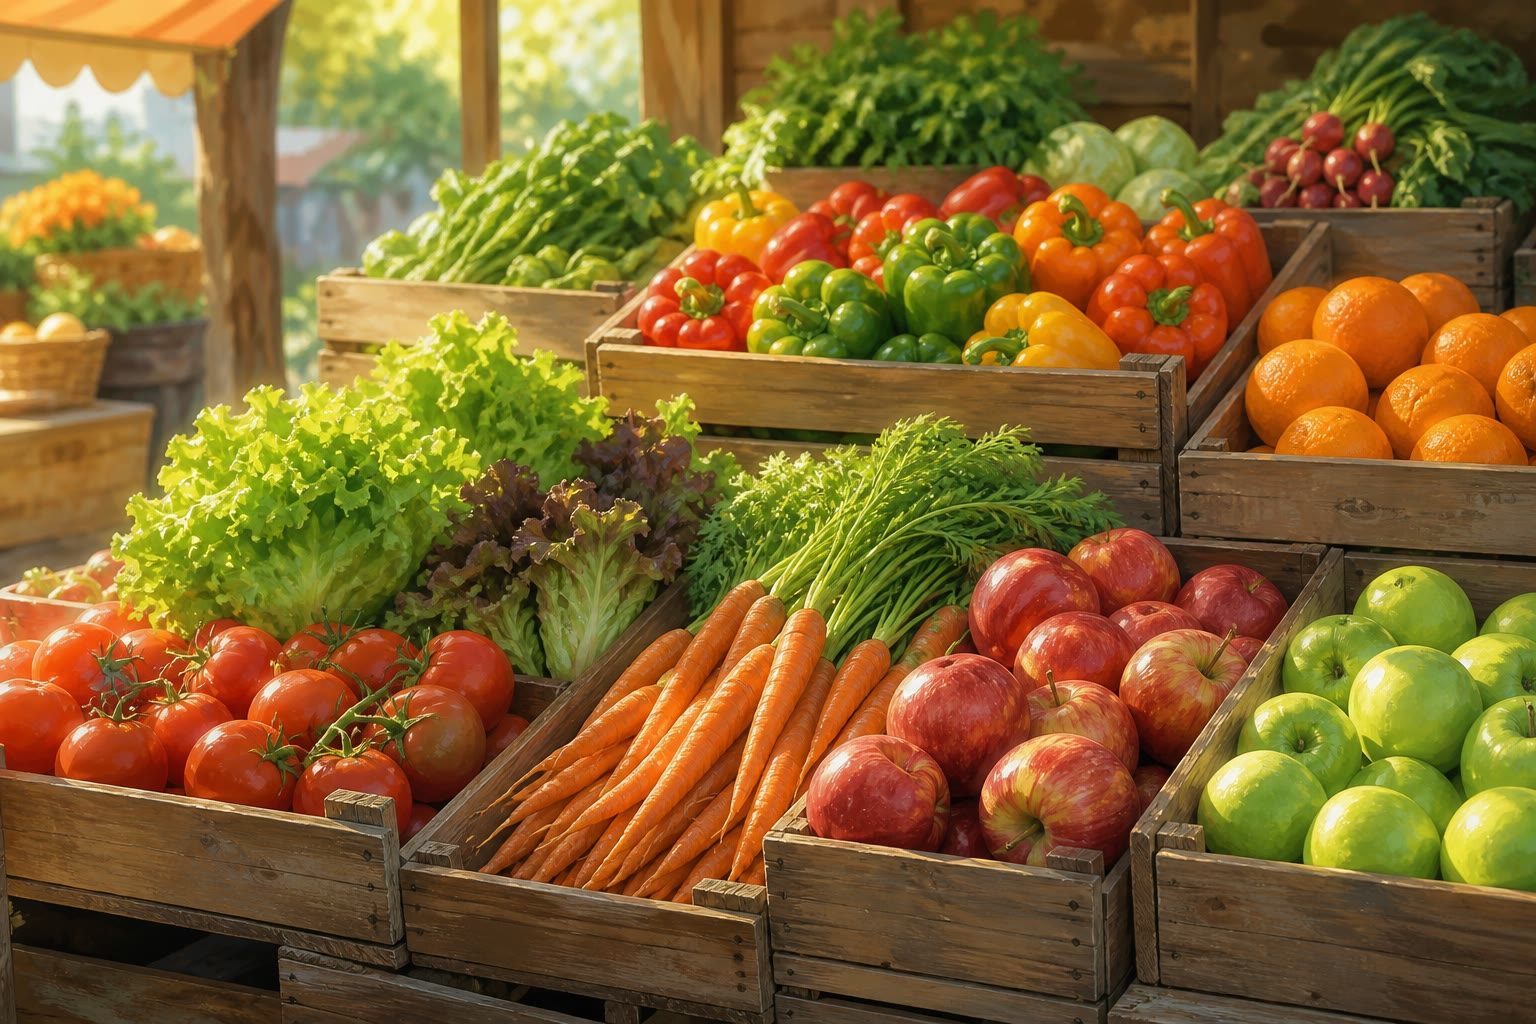
\includegraphics[width=0.62\linewidth]{images/book1/ai/g3-diet-market.jpg}

{\small 集市上的“新鲜类”：盘子中最常被遗忘的一角，
这里却绝不会被忽略。}
\end{omfigure}

\begin{omfigure}
\begin{tikzpicture}
  % plate
  \draw[thick] (0,0) circle (2.8);
  % half: vegetables/fruit
  \draw[thick, fill=omMeth!14] (0,0) -- (0,2.8)
    arc[start angle=90, end angle=270, radius=2.8] -- cycle;
  % quarter: starchy
  \draw[thick, fill=omProp!14] (0,0) -- (0,-2.8)
    arc[start angle=270, end angle=340, radius=2.8] -- cycle;
  % quarter: builders
  \draw[thick, fill=omThm!12] (0,0) -- ({2.8*cos(340)},{2.8*sin(340)})
    arc[start angle=-20, end angle=90, radius=2.8] -- cycle;
  \node[font=\small, align=center] at (-1.4,0.2)
    {水果和蔬菜 \\ （占盘子的一半）};
  \node[font=\small, align=center] at (1.0,-1.45)
    {面包、\\ 意大利面、大米};
  \node[font=\small, align=center] at (1.3,1.0)
    {肉、鱼、\\ 蛋或奶制品};
  % water glass
  \draw[thick] (4.0,-0.5) -- (4.1,1.0) -- (5.0,1.0) -- (5.1,-0.5)
    -- cycle;
  \fill[omDef!25] (4.04,-0.44) -- (4.12,0.75) -- (4.98,0.75)
    -- (5.06,-0.44) -- cycle;
  \node[font=\small, align=center] at (4.55,-1.0) {水};
\end{tikzpicture}

{\small 均衡的餐盘：一半是“新鲜类”，四分之一是稳定供能的类别，
四分之一是“建造类”——杯中还有水。}
\end{omfigure}

\begin{example}[搭配一份午餐]\label{ex:g3:balanced-diet:lunch}
番茄酱意大利面、一块鱼、四季豆、一杯酸奶，
一个苹果，再加水：各类食物齐全，没有零食——这是
一顿均衡的午餐。薯片、一瓶汽水和一块巧克力只提供两类
（脂肪和糖），却漏掉了建造工地
正在等待的那些类别。
\end{example}

\begin{remark}[没有禁止的食物，只有被遗忘的食物]\label{rem:g3:balanced-diet:balance}
平衡是按天数来衡量的，而不是看单独的几口。一块生日蛋糕
并不违反任何规则——问题从来不在于某一次零食，
而在于每天都用零食\emph{代替}各类食物。每一餐真正要问的
问题不是“这种食物坏不坏？”，而是
“今天我忘了哪一类？”
\end{remark}

\section{按一天的安排搭配食物}

\begin{proposition}[需求随一天的安排与每个人而变]\label{prop:g3:balanced-diet:needs}
身体需要多少\omterm{prop:g3:balanced-diet:jobs}{能量}，取决于它是谁、
在做什么：正在生长的儿童，相对于成年人，
需要按比例更多的建造材料；一天的运动或冬日的严寒
消耗的\omterm{prop:g3:balanced-diet:jobs}{能量}，比一个下午的阅读要多。饥饿感
随身体的消耗而增强。
\end{proposition}
\admitted

\begin{example}[早餐为什么重要]\label{ex:g3:balanced-diet:breakfast}
清晨时分，身体整夜都在运转——心脏、呼吸、
体温——却没有任何补给。早餐为它补充\omterm{prop:g3:balanced-diet:jobs}{能量}，
以应对上午的课程和奔跑玩耍。若不吃早餐，
到上午中段，身体便会供应不足：肚子咕咕叫、
注意力分散，玩耍时没有力气。
\end{example}

\begin{method}[检查一天的膳食平衡]\label{met:g3:balanced-diet:check}
一天结束时，逐条检查下面的清单：
\begin{enumerate}
  \item 每一餐都有水果或蔬菜吗？（目标：
        一天约五份）
  \item 每餐都吃淀粉类食物，以获得稳定的\omterm{prop:g3:balanced-diet:jobs}{能量}？
  \item 是否有建造材料——奶制品隔几天吃一次，肉、鱼
        或蛋吃一次或两次？
  \item 全天的饮品是水吗？
  \item 零食：只吃少量，而不是主要部分？
\end{enumerate}
缺了哪一类，明天就请它来。
\end{method}

\section{练习}

\begin{exercise}[$\star$]\label{exo:g3:balanced-diet:1}
食物有哪两项作用？请分别举出一类主要
承担每项作用的\omterm{def:g3:balanced-diet:families}{食物类别}。
\end{exercise}

\begin{exercise}[$\star$]\label{exo:g3:balanced-diet:2}
写出\omterm{def:g3:balanced-diet:families}{食物类别}，以及身体必需的那一种饮品。
\end{exercise}

\begin{exercise}[$\star$]\label{exo:g3:balanced-diet:3}
请把这些食物按类别分类：大米、酸奶、胡萝卜、鸡蛋、
黄油、苹果、面包。
\end{exercise}

\begin{exercise}[$\star$]\label{exo:g3:balanced-diet:4}
为什么身体在\omterm{prop:g1:healthy-habits:needs}{睡眠}时仍会消耗\omterm{prop:g3:balanced-diet:jobs}{能量}？写出
夜间两项\omterm{prop:g3:balanced-diet:jobs}{能量}消耗。
\end{exercise}

\begin{exercise}[$\star$]\label{exo:g3:balanced-diet:5}
对照午餐“意大利面、鱼、四季豆、酸奶、苹果、
水”与图中的平衡餐盘对照：每一项分别属于
餐盘的哪一部分？
\end{exercise}

\begin{exercise}[$\star$]\label{exo:g3:balanced-diet:6}
为什么早餐尤其重要？如果不吃早餐，
上午中段会出现什么情况？
\end{exercise}

\begin{exercise}[$\star$]\label{exo:g3:balanced-diet:7}
哪一类人按比例需要更多的建造材料：儿童还是
成年人？为什么？
\end{exercise}

\begin{exercise}[$\star$]\label{exo:g3:balanced-diet:8}
动手试一试：对自己的一天运用\cref{met:g3:balanced-diet:check}，
诚实地检查。你忘记了哪一类食物——哪一类
出现的次数超过了它应得的份额？
\end{exercise}

\begin{exercise}[$\star\star$]\label{exo:g3:balanced-diet:9}
“甜食是被禁止的！”本章真的这样说吗？请给出
\cref{rem:g3:balanced-diet:balance}中更精确的规则。
\end{exercise}

\begin{exercise}[$\star\star$]\label{exo:g3:balanced-diet:10}
在滑雪假期中，每个人都比在家时更饿。请
结合\cref{prop:g3:balanced-diet:needs}解释——
说出寒冷而多运动的一天额外增加的两项\omterm{prop:g3:balanced-diet:jobs}{能量}消耗。
\end{exercise}
